% !TeX spellcheck = en_US

Using the concept, described in Chapter \ref{sec:concept}, I were able to implement the newly designed parts of the ER model, shown in Figure \ref{fig:db-er-model}, in \neoj. These graph structures are generated by a plugin written to interface the native \neoj API on the one side and \bives on the other.
Converting this formal describe ER model into a graph database schema as shown in Figure \ref{fig:results:simple-diff}, was performed as described in Section \ref{sec:background:graph-db:er}. Despite the direct convertibility, some optimizations and adjustments for convenience were made.
Also the figure shows an simplified representation of a delta between a relatively simple toy model. The figure was reduced to maintain readability, while still illustrate the basic schema.

Nonetheless the schema was designed around a \texttt{DIFF} node, which is linked by a \texttt{HAS\_DIFF} relation, from two consecutive versions of the same model. These two versions are again linked with the \texttt{HAS\_SUCCESSOR} and \texttt{HAS\_PREDECESSOR} relations.
The successor and predecessor relations define the version history, whereby the \texttt{DIFF} node clearly indicates the delta between those versions. The \texttt{diffPart} attribute of the \texttt{HAS\_DIFF} relations specify the direction of the delta, and therefore the role of participating \texttt{DOCUMENT} nodes. In accordance to the ER model, the role can either be \emph{source} or \emph{destination}.
These terms were chosen, due to their expressiveness in regards to temporal aspects. Otherwise an implication of order, like terms as \emph{old} and \emph{new} suggest, may cause confusion in case of reverse deltas or deltas between completely different models.

However, the central \texttt{DIFF} node links to various \texttt{DIFF\_NODE}s, using the \texttt{HAS\_DIFF\_ENTRY} relation. Since \neoj supports multiple labels per node, the 4 change types \texttt{DIFF\_INSERT}, \texttt{DIFF\_DELETE}, \texttt{DIFF\_UPDATE}, and \texttt{DIFF\_MOVE} can be grouped together using an additional label \texttt{DIFF\_NODE}. This simplifies queries and will eventually steed them up as well, due to having a single index for all change types.
Any kind of \texttt{DIFF\_NODE} might link to any node beneath the \texttt{DOCUMENT} node in at least on of the 2 compared models, in correspondence to the type of change.
As illustrated by the \texttt{DIFF\_UPDATE} node in Figure \ref{fig:results:simple-diff} (small yellow node, labeled with a \emph{2}). On one hand it connects to the species \emph{A} in the \emph{source} model version using the \texttt{IS\_SOURCE} relation. On the other hand it also connects to the updated counterpart, which is the species \emph{A} in the \emph{destination} version using the \texttt{IS\_DESTINATION} relation.
Furthermore a causality chain among changes is expressed, by the \texttt{DIFF\_TRIGGERED\_BY} relation, which points from one \texttt{DIFF\_NODE} to another. This is illustrated by the \texttt{DIFF\_INSERT}, labeled with the number \emph{3}, in Figure \ref{fig:results:simple-diff}. This insert caused 4 other inserts, describing the insertion of id, name, compartment reference, and initial concentration.

In addition to these structural information each \texttt{DIFF\_NODE} contains among other all attributes \bives assigns to a change. These \bives specific information include a XPath expressions, locating a change in both versions, values of \emph{source} and \emph{destination} in case of an attribute change, name and id of the changed element, as well as a possible reference to change, that triggered this current one.
Besides the \bives attributes, the \texttt{DIFF\_NODE} contains another important marker as attribute.
The \texttt{inherit} flag indicates, if a change detected by \bives, does not have a direct match in \masymos's graph structure. Instead the model structure is traversed  upwards, until a element is found having a representation in the \masymos graph.
This, for instance, applies to changes of a mathematical parameter in a kinetic law of a reaction. In this specific example, the change would be linked to the node representing the reaction, since mathematical structures or kinetic laws are not represented by nodes in \masymos. Another example would be text nodes of any kind, which are stored within a Lucene index by \masymos, but not in the graph representation, since they are not an essential part of the models structure.
The \texttt{inherit} flag consequently allows to store and analyze changes, which otherwise could not be integrated into the schema.

Furthermore \texttt{DIFF\_NODE}s might link to multiple \comodi terms. \comodi's entire reasoned taxonomy is stored in \masymos, so queries matched against more abstract terms also include references to more specialized terms. The resulting network is shown in Appendix \ref{fig:appendix:neo4j-comodi}.
Before generating any deltas the \comodi ontology needs to be imported initially. Otherwise terms might be created on occurrence, but not interlinked according to the taxonomy.
The initial import is performed using mostly already existing mechanisms in \masymos, which were only adjusted, so they can work with dynamic ontology names (cf. Section \ref{sec:impl:masymos}). In this process the ontology is first of all loaded in its \owl representation and then validated with the Hermit\footnote{\todo{find resource to hermit}} reasoner. The second step not only makes sure only logically correct ontologies are imported, but also to import the \emph{inferred} ontology. This takes away logical classification steps, when querying for abstract ontology classes.

The import of actual models, however, is performed by the \modelcrawler (cf. Section \ref{sec:impl:modelcrawler}), resulting in a \masymos database filled with all model versions of \emph{BioModels Database} and \emph{PMR2} (cf. Section \ref{sec:background:modelrepo}) and a hierarchical file structure containing all original files, complying with the model described in Section \ref{sec:concept:filestorage}.
During a test run, done at ???, this resulted in \todo{add some fancy numbers here}.

On the contrary, models for test purposes and to generate Figure \ref{fig:results:simple-diff} were imported using a small Python\footnote{\todo{link to Python?}} script. This script emulates a HTTP daemon, while simultaneously sending import commands to the \masymos \rest interface \morre. Using this script eases the process of importing test data, since neither the \modelcrawler needs to be configure, nor a sane folder structure needs to be build manually.
import!



\todo{what's done from the concept}
\todo{still high-level}
\todo{what problem is solved?}

\begin{itemize}
	\item implemented db concept
		\subitem picture from simple-sbml-demo
		\subitem rest of pictures in appendix
	\item Ontology import
		\subitem changes to \masymos core
		\subitem using existing import mechanics, but dynamic
	\item http server storage concept?
\end{itemize}



solved:
"A model VCS should be tailored to existing model representation formats, which are typically XML and RDF based. It should furthermore reflect the temporal evolution of a model and present model changes to the users." \citep{Waltemath2013}

The objective of this thesis is therefore to investigate into a concept to store systems biology models in a way, that multiple versions can be accessed, queried, and compared. Further, semantical annotations of changes between these versions shall be introduced. These additional relations are meant to improve the ability to query for a version of a model by specific criteria and consequently improving the user experience for biologists seeking to build onto existing models, as the evolution of them plays an important role for them \citep{Scharm2015}

\begin{figure}
	\centering
	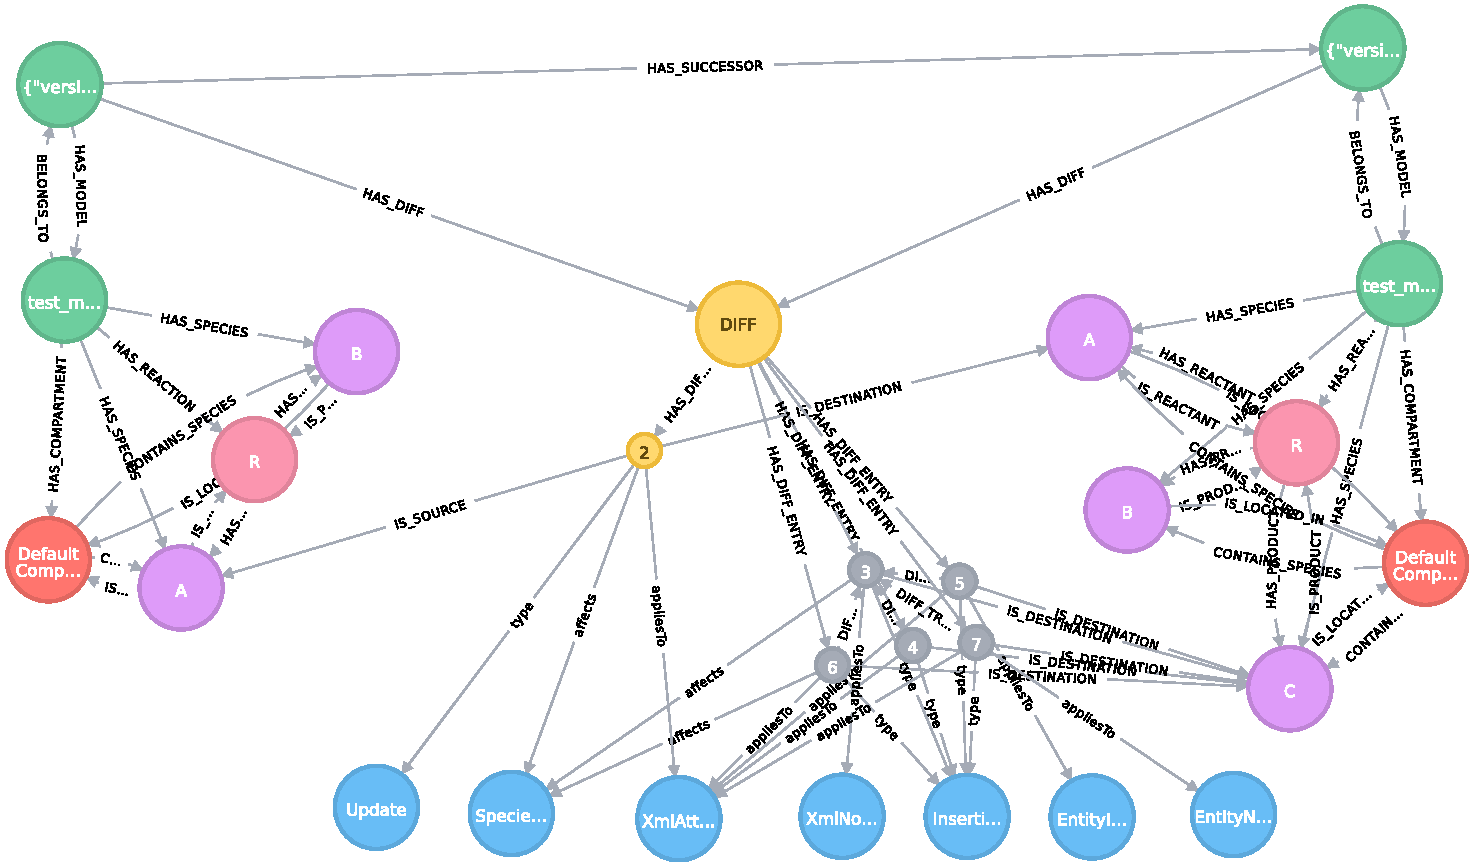
\includegraphics[width=\textwidth]{resources/neo4j-renders/demo-sbml-simple-diff.pdf}
	\caption[Reduced representation of a delta in \masymos, between two versions of a the simple \sbml demo model]{Reduced representation of a delta in \masymos, between two versions of a the simple \sbml demo model. The delta, organized around the \texttt{DIFF} node, only shows changes, with a direct match in the graph representation. Further most up traversing relations are not shown, to increase readability.}
	\label{fig:results:simple-diff}
	
\end{figure}